\documentclass[a4paper]{scrreprt}
\usepackage{fancyhdr}
\pagestyle{fancy}
\usepackage[english]{babel}
\usepackage[utf8]{inputenc}
\usepackage{graphicx}
\usepackage{url}
\usepackage{textcomp}
\usepackage{amsmath}
\usepackage{lastpage}
\usepackage{pgf}
\usepackage{wrapfig}
\usepackage{fancyvrb}
\usepackage{pdfpages}

\usepackage{etoolbox}
\makeatletter
\patchcmd{\scr@startchapter}{\if@openright\cleardoublepage\else\clearpage\fi}{}{}{}
\makeatother

\usepackage[colorlinks=true, linkcolor=violet]{hyperref} %links with \href{}
\usepackage[figure]{hypcap} %jump to img instead of caption

\newcommand{\code}[1]{\texttt{#1}}

% Create header and footer
\headheight 27pt
\pagestyle{fancyplain}
\lhead{\footnotesize{Applikationer för internet, ID1354}}
\chead{\footnotesize{Assignment 3 report}}
\rhead{}
\lfoot{}
\cfoot{\thepage\ (\pageref{LastPage})}
\rfoot{}

% Create title page
\title{Assignment 3}
\subtitle{Applikationer för internet, ID1354}
\author{Max Körlinge, korlinge@kth.se}
\date{\today}

\begin{document}

\maketitle

\tableofcontents %Generates the TOC
\clearpage

\chapter{Introduction}

This assignment concerns structuring the web application to follow the MVC pattern, and to implement three security measures from a list. Optional tasks were to use a database to store data, and to improve performance. I chose to use a database, but not improve performance. For the mandatory task 1 I chose to implement the MVC architecture without using a framework.

\chapter{Literature Study}

To complete the tasks I first studied the course lecture notes on MVC for a web application and web security.

\chapter{Method}

\section{Task 1a}
I started trying to "happy hack" my way through this assignment but quickly realized that I had to have a plan, so I started off by making a class diagram in Astah-community. I started by implementing all actions a user could take as a function in the Controller, and then added operations and other classes as I saw fit. After the MVC diagram was finished I coded each action one by one (for example first logging in a user, then registering a user, then writing a comment, etc), changing the class diagram when necessery. I use view, controller, model, and integration layers. The view layer has all pages, HTTP requests, and parts that are included in the views, such as header and footer. All the other layers are pure PHP classes that are called from the view (through the controller). To make objects persist I made the Controller destruct method serialize the controller in the session cookie.

\section{Task 2}

I chose to implement File Security. Apache2 works as a user who only deals with the webroot (www-data), and when working with the site I use a small bash script that copies the files into the web root, and then sets \code{chmod -R 755} on the directories, which means that only root user has access to changing the files, all other users, such as the apache user, can only read and execute files inside. I also denied HTTP access to all files containing PHP classes through the apache configuration.

I also chose to implement database security. I had already set up my mySQL database so that a special user was created who only had access to the database pertaining to the website. I then changed all the methods in the integration layer class \code{DatabaseRequest}, which handles database requests, to use parameterized requests using \code{prepare()} and \code{execute()}, instead of the \code{query()} method I was using before.

At last I chose to implement password encryption. Since I first restructured the program to use the MVC architecture, I could simply change the \code{loginUser()} and \code{registerNewUser()} methods in the \code{UserAccountHandler} class to use \code{password\_hash} and \code{password\_verify} PHP functions instead of storing the password as plain text.

\section{Optional Task 1}

I actually chose to use a database already in the last assignment. To set up the database quickly on different servers when I change environment, I wrote a sql file that does this if you source it from the mySQL command line. You can find it at \href{https://github.com/fongie/TastyRecipes/blob/assignment3/res/sql/initDB.sql}{this link}. I then use SQL queries and the PDO library to fetch and insert data into the database.

\chapter{Result}
\label{sec:result}

The git repository can be found \href{https://github.com/fongie/TastyRecipes/tree/assignment3}{here}.

\section{Task 1}

All source code is inside the \code{src} directory, where the layers are: \code{controller}, \code{model}, \code{integration}, and \code{util}. Inside each map are the class files, one file per class. The structure is best described by the class diagram in Figure \ref{fig:classdia}. There is only mixed PHP and HTML in the \code{view} layer, all other code is object oriented PHP. There are only three static methods: two in the \code{Util} class used by the \code{view} layer for redirections, and one, also used by the view, for getting the \code{Controller} from the \code{SESSION} cookie. All layers have the roles specified by the MVC pattern, and there are only dependencies "downwards" through the layers, as can be seen in the class diagram.

\begin{figure}[h!]
  \begin{center}
    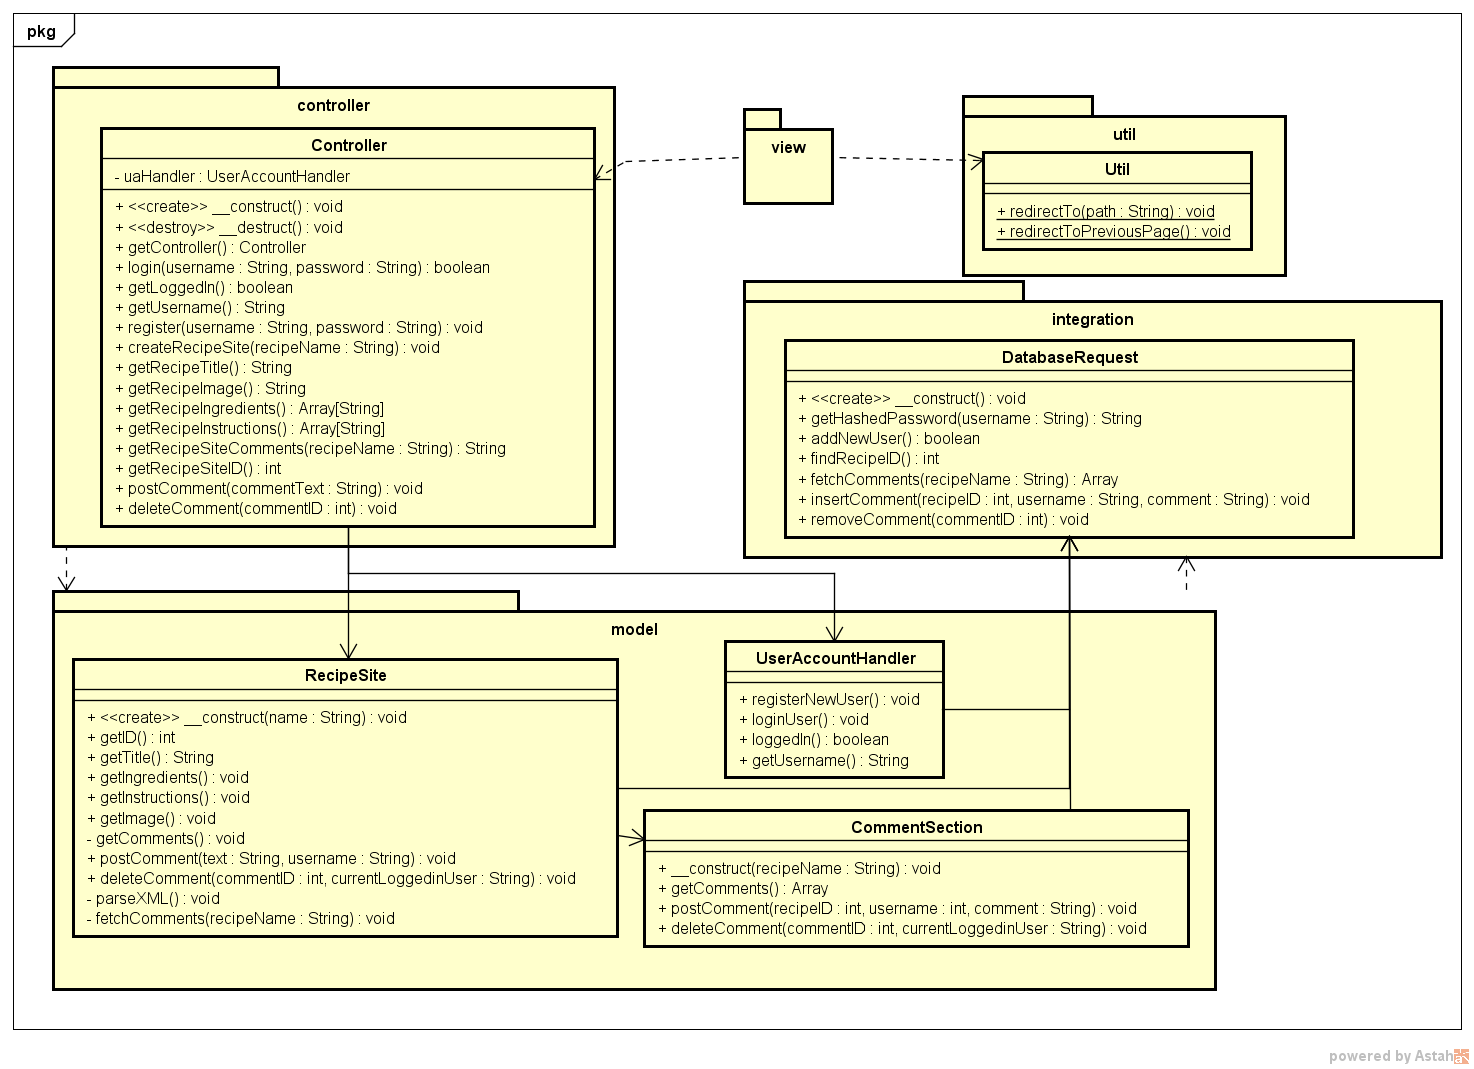
\includegraphics[scale=0.41]{img/TastyRecipesMVC.png}
    \caption{A class diagram describing the Tasty Recipes web application}
    \label{fig:classdia}
  \end{center}
\end{figure}

\section{Task 2}
I do not use HTTPS but HTTPS should be used whenever HTTP requests are being made by an authenticated user such as logging in, registering, or posting or deleting comments.

The file security of the system is strong on the webserver, as seen in Figure \ref{fig:ownership} and Figure \ref{fig:reqaccess}.

\begin{figure}[h!]
  \begin{center}
    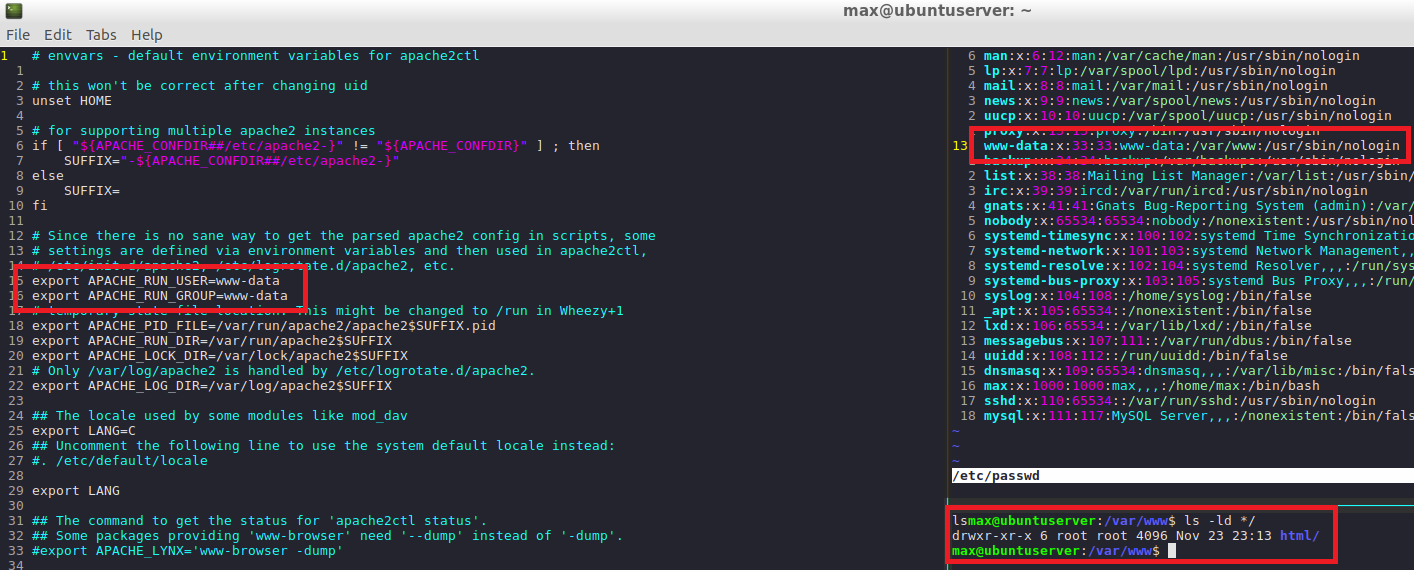
\includegraphics[scale=0.41]{img/filesecurity_ownership.png}
    \caption{Files showing apache username and web root file access.}
    \label{fig:ownership}
  \end{center}
\end{figure}

\begin{figure}[h!]
  \begin{center}
    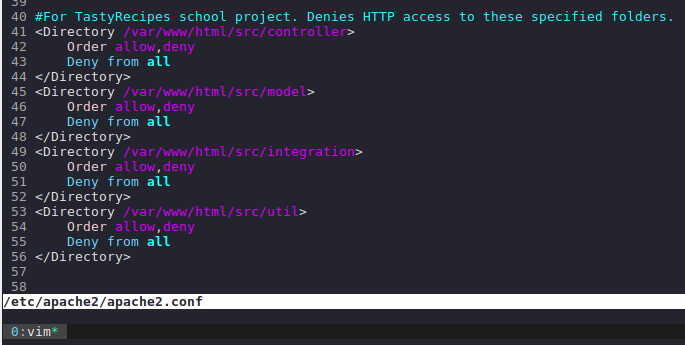
\includegraphics[scale=0.41]{img/filesecurity_reqaccess.png}
    \caption{The apache2 config file restricting HTTP access to all layers except the view}
    \label{fig:reqaccess}
  \end{center}
\end{figure}

Database security is maintained on the mySQL server using a unique user for the webapp, and by using parameterized queries in all requests to the database, as seen in \href{https://github.com/fongie/TastyRecipes/blob/assignment3/src/integration/DatabaseRequest.php}{this class file}.

Usage of password encryption can be seen \href{https://github.com/fongie/TastyRecipes/blob/86f4548c3b4659b762134c756cc5ac4c0cbf72a2/src/model/UserAccountHandler.php#L35}{here} and \href{https://github.com/fongie/TastyRecipes/blob/86f4548c3b4659b762134c756cc5ac4c0cbf72a2/src/model/UserAccountHandler.php#L18}{here}.

\section{Optional Task 2}

Database requests are made using the PDO library and SQL queries. All requests are made using a new instance of the \code{DatabaseRequest} class. The easiest way to see how data is inserted and extracted is to see the code for that class, \href{https://github.com/fongie/TastyRecipes/blob/assignment3/src/integration/DatabaseRequest.php}{here}.

\chapter{Discussion}

Implementing the MVC architecture from completely unstructured code was a long process and not very easy at first, the result is however a clear impementation of the MVC architecture. It helped tremendously to plan ahead using a class diagram. There are some requests that are passed down quite a long way, for example through the \code{Controller}, through a \code{RecipeSite} all the way to a \code{CommentSection}, but this is to reduce coupling on the \code{Controller} which now only has dependencies on two classes. All layers are well encapsulated, since all calls are made from the top and downwards. The \code{Util} class could have been left out but redirecting pages was so frequent in the view that I wanted to make a class for it. Since there were not many classes and files in this webapp I decided not to use a class autoloader. It makes it easier to keep track of what is actually imported, perhaps keeping a likeness to Java. Each import is required once instead.

The security implementations were straightforward following the instructions in the lecture notes, there is not much to discuss about that.

\chapter{Comments About the Course}

I spent more than 40 hours on this assignment.
As predicted after the previous assignment, structuring the code was a lot of work, despite having done the Object Oriented Design course last semester.
Implementing security was easy, especially using a linux web server.

\end{document}
